\section{Correction de la résolution en énergie avec les événements \Gjets}\label{chapter-JERC-section-JER}
Déterminer la correction de la résolution en énergie des jets, ou JER, en 2018 et 2017-UL avec les événements \Gjets\ a été un des mes travaux de thèse.
La méthode est sensiblement la même que pour déterminer la correction résiduelle absolue en \pT\ des jets, ou JES.
\par Dans le cas de la JES, la moyenne de la distribution des réponses des jets est corrigée. Pour la JER, c'est la largeur de cette distribution qui doit être corrigée.
La sélection des événements est ainsi faite comme dans le cas de la JES décrite section~\ref{chapter-JERC-section-JES-subsec-evt_select}, à ceci près que la correction résiduelle absolue en \pT\ des jets est appliquée.
\subsection{Définition de la résolution en énergie des jets}\label{chapter-JERC-section-JER-subsec-JER_definition}
La résolution en énergie des jets se détermine à l'aide de leur réponse balancée \Rbal.
À partir de la définition de \Rbal\ en page~\pageref{eq-chapter-JERC-section-CMS-subsec-residuals-Rbal_def}, il est possible d'écrire dans le cas des événements \Gjets
\begin{equation}
\Rbal
= \frac{\pT_\reco^\text{jet 1}}{\pT^{\photon}}
= \frac{\pT_\reco^\text{jet 1}}{\pT^{\photon}_\reco}
=
\frac{\pT_\reco^\text{jet 1}}{\pT^\text{jet 1}_\ptcl}
\times
\frac{\pT^\text{jet 1}_\ptcl}{\pT^{\photon}_\ptcl}
\times
\frac{\pT^{\photon}_\ptcl}{\pT^{\photon}_\reco}
\mend[,]
\end{equation}
ce qui se traduit en terme des largeurs des distributions de chacune de ces fractions sous la forme
\begin{equation}
\sigma_{\Rbal}
=
\sigma\left(\frac{\pT_\reco^\text{jet 1}}{\pT^\text{jet 1}_\ptcl}\right)
\oplus
\sigma\left(\frac{\pT^\text{jet 1}_\ptcl}{\pT^{\photon}_\ptcl}\right)
\oplus
\sigma\left(\frac{\pT^{\photon}_\ptcl}{\pT^{\photon}_\reco} \vphantom{\frac{\pT^\text{jet 1}_\ptcl}{\pT^{\photon}_\ptcl}}\right)
\label{eq-sigmas_quadratic_sum_1}
\mend[,]
\end{equation}
où $\oplus$ désigne une somme quadratique.
Des termes de cette dernière équation, le premier rend compte de la résolution en énergie des jets au niveau reconstruit et est noté $\sigma_\text{JER}$ dans la suite.
Il s'agit de la grandeur d'intérêt dans cette analyse.
Le second terme est lié à la physique de l'événement sous-jacent, \ie\ de l'empilement, des radiations et des neutrinos.
Après extrapolation vers $\alpha=0$, la contribution des radiations devient négligeable.
Ce terme est noté $\sigma_\text{PLI}$ dans la suite; \og PLI \fg{} signifie interaction au niveau particule (\emph{Particle Level Interaction}).
Enfin, le dernier terme est lié à la résolution en énergie des photons, noté $\sigma_{\photon}$.
\par L'équation~\eqref{eq-sigmas_quadratic_sum_1} se réécrit alors, en utilisant les notations introduites,
\begin{equation}
\sigma_{\Rbal}
=
\sigma_\text{JER}
\oplus
\sigma_\text{PLI}
\oplus
\sigma_{\photon}
\label{eq-sigmas_quadratic_sum_2}
\mend[,]
\end{equation}
ce qui peut se réarranger afin d'exprimer $\sigma_\text{JER}$ sous la forme
\begin{equation}
\sigma_\text{JER}
=
\sigma_{\Rbal}
\ominus
\sigma_\text{PLI}
\ominus
\sigma_{\photon}
\label{eq-sigmas_quadratic_sum_3}
\mend
\end{equation}
La bonne qualité de reconstruction des photons permet de négliger le terme $\sigma_{\photon}$ dans la suite.
\subsection{Analyse}\label{chapter-JERC-section-JER-subsec-analyse}
\paragraph{Similitudes avec l'analyse menée pour la JES}
L'analyse des événements \Gjets\ dans le cas de la JER est semblable à celle pour la JES, décrite dans la section~\ref{chapter-JERC-section-JES-subsec-analyse}.
Les intervalles de $\pT^{\photon}$, $\abs{\eta^\text{jet}}$ et $\alpha$ sont toutefois différents.
Les intervalles de ces grandeurs utilisés pour la JER sont définis dans les tableaux~\ref{tab-pT_photon_intervalles-JER}, \ref{tab-eta_jet_intervalles_fin-JER} et~\ref{tab-alpha_intervalles-JER}.
En particulier, les intervalles de $\alpha$ sont exclusifs, contrairement aux intervalles inclusifs utilisés pour la JES.
\begin{table}[h]
\centering
\begin{tabular}{ccccc}
\toprule
$[\num{105}, \num{130}[$ & $[\num{130}, \num{175}[$ & $[\num{175}, \num{200}[$ & $[\num{200}, \num{230}[$ & $[\num{230}, \num{300}[$ \\
$[\num{300}, \num{400}[$ & $[\num{400}, \num{500}[$ & $[\num{500}, \num{700}[$ & $[\num{700}, \num{3000}[$ \\
\bottomrule
\end{tabular}
\caption[Intervalles de $\pT^{\photon}$ utilisés pour la JER.]{Intervalles de $\pT^{\photon}$ en \SI{}{\GeV} utilisés pour la JER.}
\label{tab-pT_photon_intervalles-JER}
\end{table}
\begin{table}[h]
\centering
\begin{tabular}{ccccc}
\toprule
$[\num{0.0}\isp \num{0.522}[$ & $[\num{0.522}\isp \num{0.783}[$ & $[\num{0.783}\isp \num{1.131}[$ & $[\num{1.131}\isp \num{1.305}[$ & $[\num{1.305}\isp \num{1.740}[$ \\
$[\num{1.740}\isp \num{1.930}[$ & $[\num{1.930}\isp \num{2.043}[$ & $[\num{2.043}\isp \num{2.322}[$ & $[\num{2.322}\isp \num{2.5}[$ & $[\num{2.5}\isp \num{2.853}[$ \\
 & $[\num{2.853}\isp \num{2.954}[$ & $[\num{2.954}\isp \num{3.139}[$ & $[\num{3.139}\isp \num{5.191}[$ &  \\
\bottomrule
\end{tabular}
\caption{Intervalles fins de $\abs{\eta^\text{jet}}$ utilisés pour la JER.}
\label{tab-eta_jet_intervalles_fin-JER}
\end{table}
\begin{table}[h]
\centering
\begin{tabular}{ccccc}
\toprule
$[\num{0}\isp \num{0.10}[$ & $[\num{0.10}\isp \num{0.15}[$ & $[\num{0.15}\isp \num{0.20}[$ & $[\num{0.20}\isp \num{0.25}[$ & $[\num{0.25}\isp \num{0.30}[$ \\
\bottomrule
\end{tabular}
\caption{Intervalles de $\alpha$ utilisés pour la JER.}
\label{tab-alpha_intervalles-JER}
\end{table}
\paragraph{Obtention de $\sigma_\Rbal$ et $\sigma_\text{PLI}$ pour $(\pT^{\photon}, \eta^\text{jet}, \alpha)$ donnés}
Pour chaque domaine
de $\pT^{\photon}$ défini dans le tableau~\ref{tab-pT_photon_intervalles-JER},
de $\eta^\text{jet}$ défini dans le tableau~\ref{tab-eta_jet_intervalles_fin-JER} et
de $\alpha$ défini dans le tableau~\ref{tab-alpha_intervalles-JER},
les distributions de la réponse balancée dans les données et les simulations sont déterminées.
\par Comme dans le cas de la JES, seuls les centres de ces distributions sont considérés afin de limiter les effets des leurs queues.
Alors, $\sigma_{\Rbal}$ s'obtient à partir des points restant comme étant le rapport de la variance de la distribution de ces points divisée par leur valeur moyenne.
\par
Dans ces mêmes domaines de $\pT^{\photon}$, $\eta^\text{jet}$ et $\alpha$, les distributions de $\pT^\text{jet 1}_\ptcl$ et $\pT^{\photon}_\ptcl$ sont estimées à partir des événements simulés.
Il est alors possible d'obtenir $\sigma_\text{PLI}$.
\paragraph{Extrapolation vers $\alpha=0$}
Une extrapolation vers $\alpha=0$ est réalisée afin de s'affranchir des effets radiatifs et de l'activité additionnelle des jets\footnote{Ces effets sont décrits dans la section~\ref{chapter-JERC-section-pheno-GJets-subsec-effets_radiatifs}.}.
Les intervalles de $\alpha$ utilisés pour la JER sont présentés dans le tableau~\ref{tab-alpha_intervalles-JER}.
L'extrapolation n'est plus linéaire comme dans le cas de la JES.
Une fonction de la forme
\begin{equation}
\sigma_i = \sqrt{(a_i\alpha)^2+b_i^2}
\end{equation}
est utilisée pour $\sigma_\Rbal^\text{données}$, $\sigma_\Rbal^\text{simulations}$ et $\sigma_\text{PLI}$.
L'extrapolation est illustrée sur la figure~\ref{fig-chapter-JERC-section-JER-subsec-analyse-resolution_eta0005_ptPhot_700_3000_extrap}.
\paragraph{Détermination de $\sigma_\text{JER}$ en fonction de $\eta^\text{jet}$}
Dans chacun des intervalles de $\pT^{\photon}$ et $\eta^\text{jet}$, pour les données et les simulations, la contribution estimée de l'événement sous-jacent est soustraite en quadrature à $\sigma_{\Rbal}$ afin d'obtenir $\sigma_\text{JER}$ en suivant l'équation~\eqref{eq-sigmas_quadratic_sum_3}.
Puis, un ajustement constant en \pT\ des rapports de $\sigma_\text{JER}$ extrapolés à $\alpha=0$ entre données et simulations est déterminé dans chaque intervalle de $\eta^\text{jet}$, comme sur la figure~\ref{fig-chapter-JERC-section-JER-subsec-analyse-resolution_eta0005_extrapolated}.
La valeur de cet ajustement correspond au facteur à appliquer à la JER dans l'intervalle de $\eta^\text{jet}$.
\begin{figure}[h]
\centering
\subcaptionbox{Extrapolation vers $\alpha=0$ de la résolution des jets pour $\abs{\eta}<\num{0.52}$ et $\num{700}<\pT^{\photon}<\SI{3000}{\GeV}$ en 2018.\label{fig-chapter-JERC-section-JER-subsec-analyse-resolution_eta0005_ptPhot_700_3000_extrap}}[.45\textwidth]
{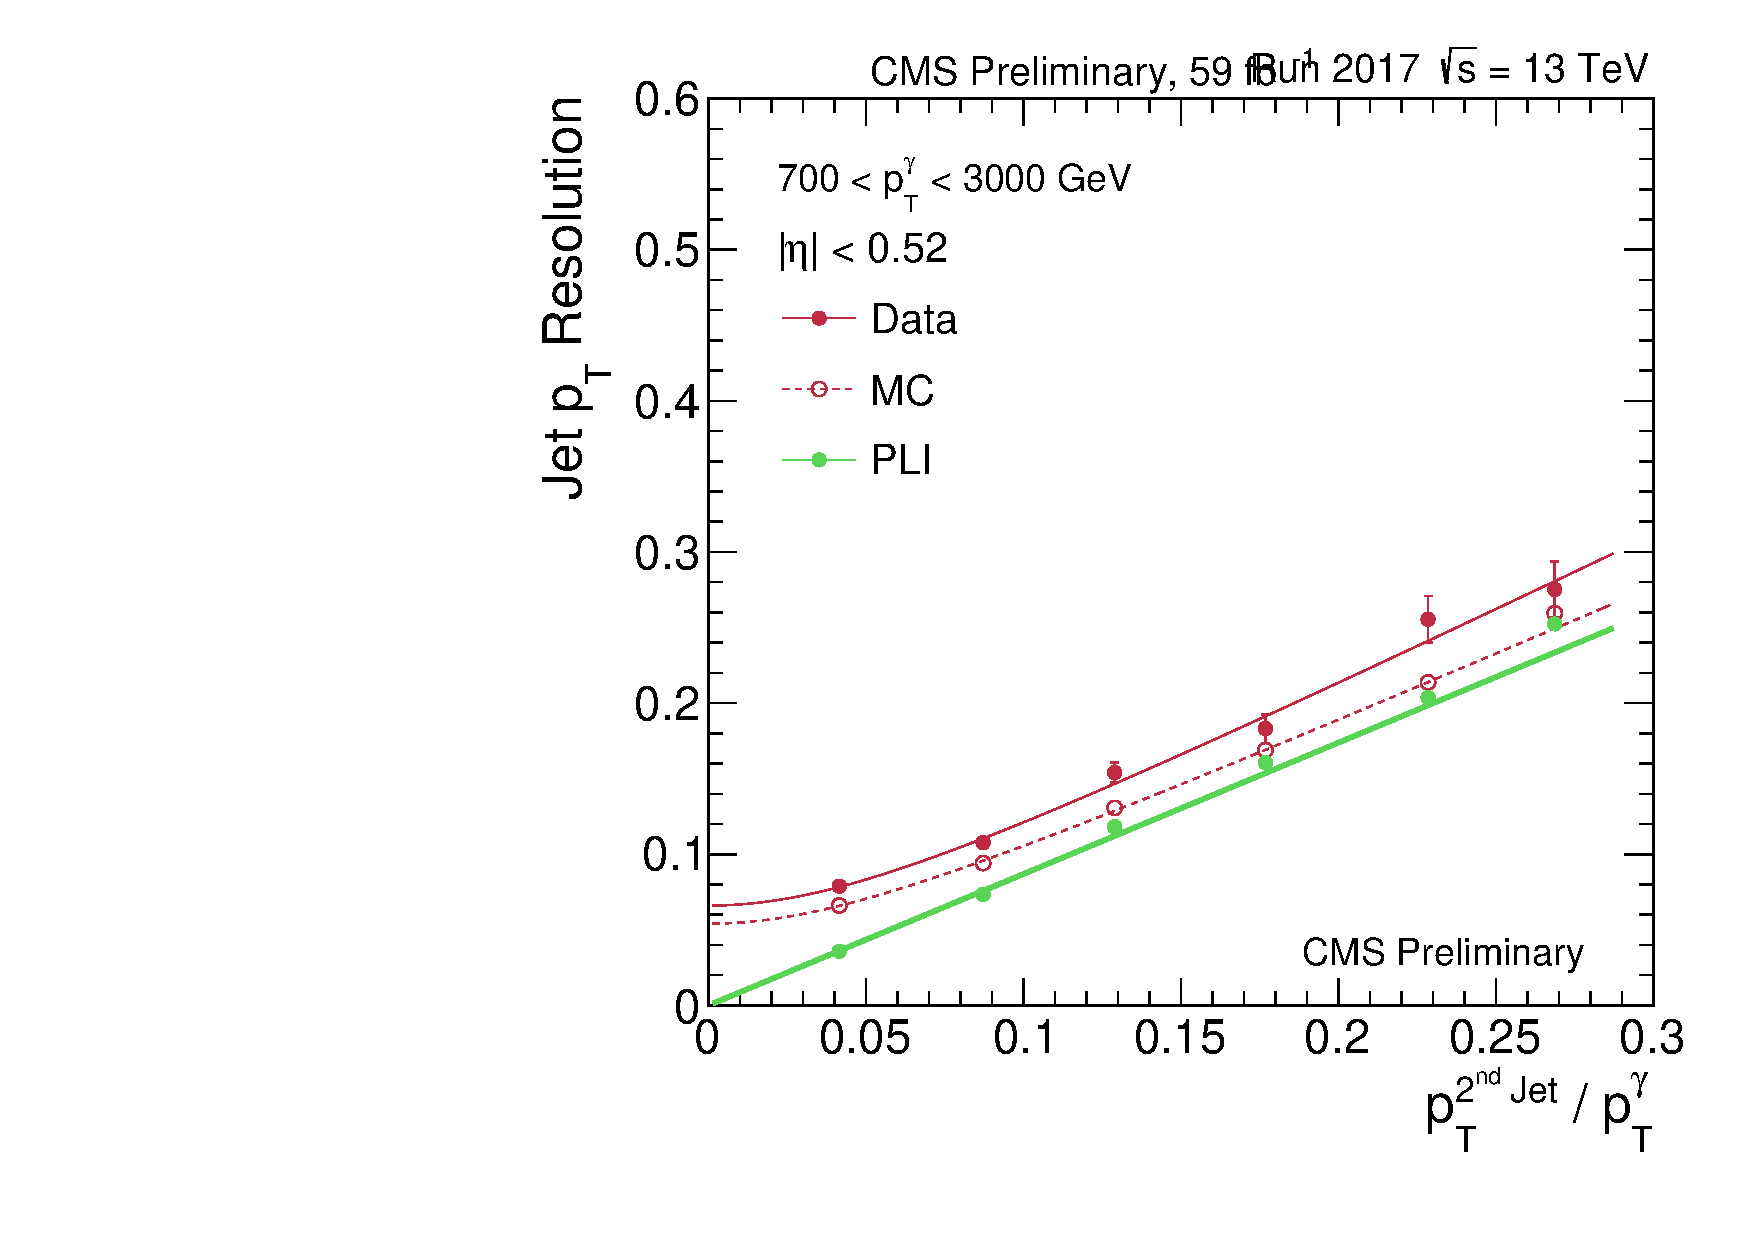
\includegraphics[width=.45\textwidth]{\PhDthesisdir/plots_and_images/my_plots/JERC/JER/Run2018ABCD/extrapolation/resolution_eta0005_ptPhot_700_3000.tex}}
\hfill
\subcaptionbox{Résolution en énergie des jets extrapolée à $\alpha=0$ pour $\abs{\eta}<\num{0.52}$ en 2018.\label{fig-chapter-JERC-section-JER-subsec-analyse-resolution_eta0005_extrapolated}}[.45\textwidth]
{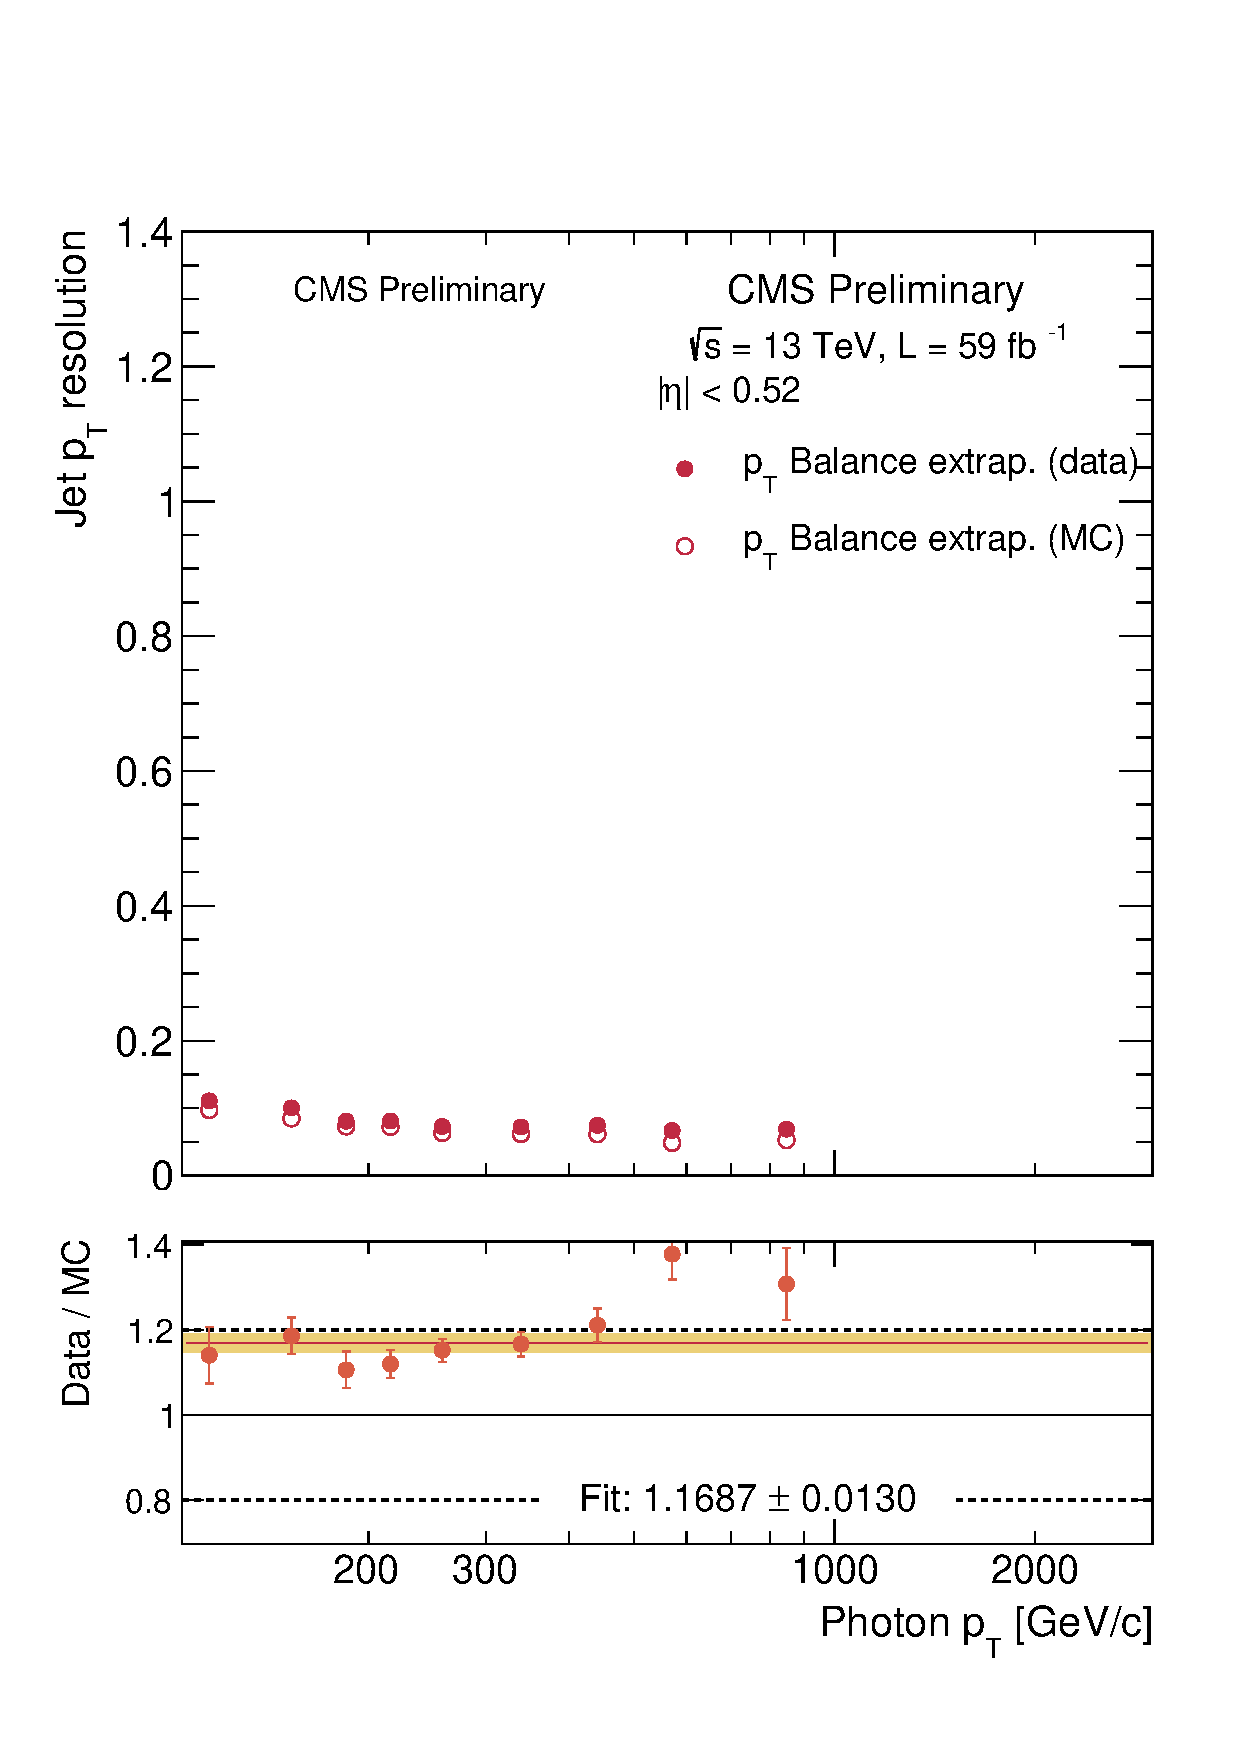
\includegraphics[width=.45\textwidth]{\PhDthesisdir/plots_and_images/my_plots/JERC/JER/Run2018ABCD/extrapolated/resolution_eta0005_balancing_extrap.pdf}}

\caption{Détermination de la résolution en énergie des jets.}
\end{figure}
\paragraph{Incertitudes}
Les incertitudes prises en compte dans la mesure de la JER sont:
\begin{itemize}
\item \SI{4.6}{\%} sur la section efficace de collision inélastique \proton\proton\ utilisée pour estimer les profils d'empilement;
\item les incertitudes de la JEC, décrites section~\ref{chapter-JERC-section-CMS-subsec-unc}, page~\pageref{chapter-JERC-section-CMS-subsec-unc}.
\end{itemize}
Les incertitudes sur l'échelle en énergie des photons ainsi que leur résolution sont négligées face aux autres incertitudes considérées.
\subsection{Résultats}\label{chapter-JERC-section-JER-subsec-results}
Les résultats issus de l'analyse des événements \Gjets\ pour l'année 2018 sont présentés sur la figure~\ref{fig-chapter-JERC-section-JER-subsec-results-fine_eta_binning_Scale_factor_res_vs_ETA}.
La combinaison avec l'analyses des événements dijet permet d'obtenir les facteurs correctifs utilisés par la collaboration, présentés sur la figure~\ref{fig-chapter-JERC-section-JER-subsec-results-CMS-DP-2020-019-JER_SF_RunII}.
Ces facteurs sont de l'ordre de \num{1.2} dans le barillet et peuvent atteindre \num{2.3} dans les bouchons.
\begin{figure}[h]
\centering
\subcaptionbox{Facteurs correctifs déterminés avec les événements \Gjets\ en 2018.\label{fig-chapter-JERC-section-JER-subsec-results-fine_eta_binning_Scale_factor_res_vs_ETA}}[.45\textwidth]
{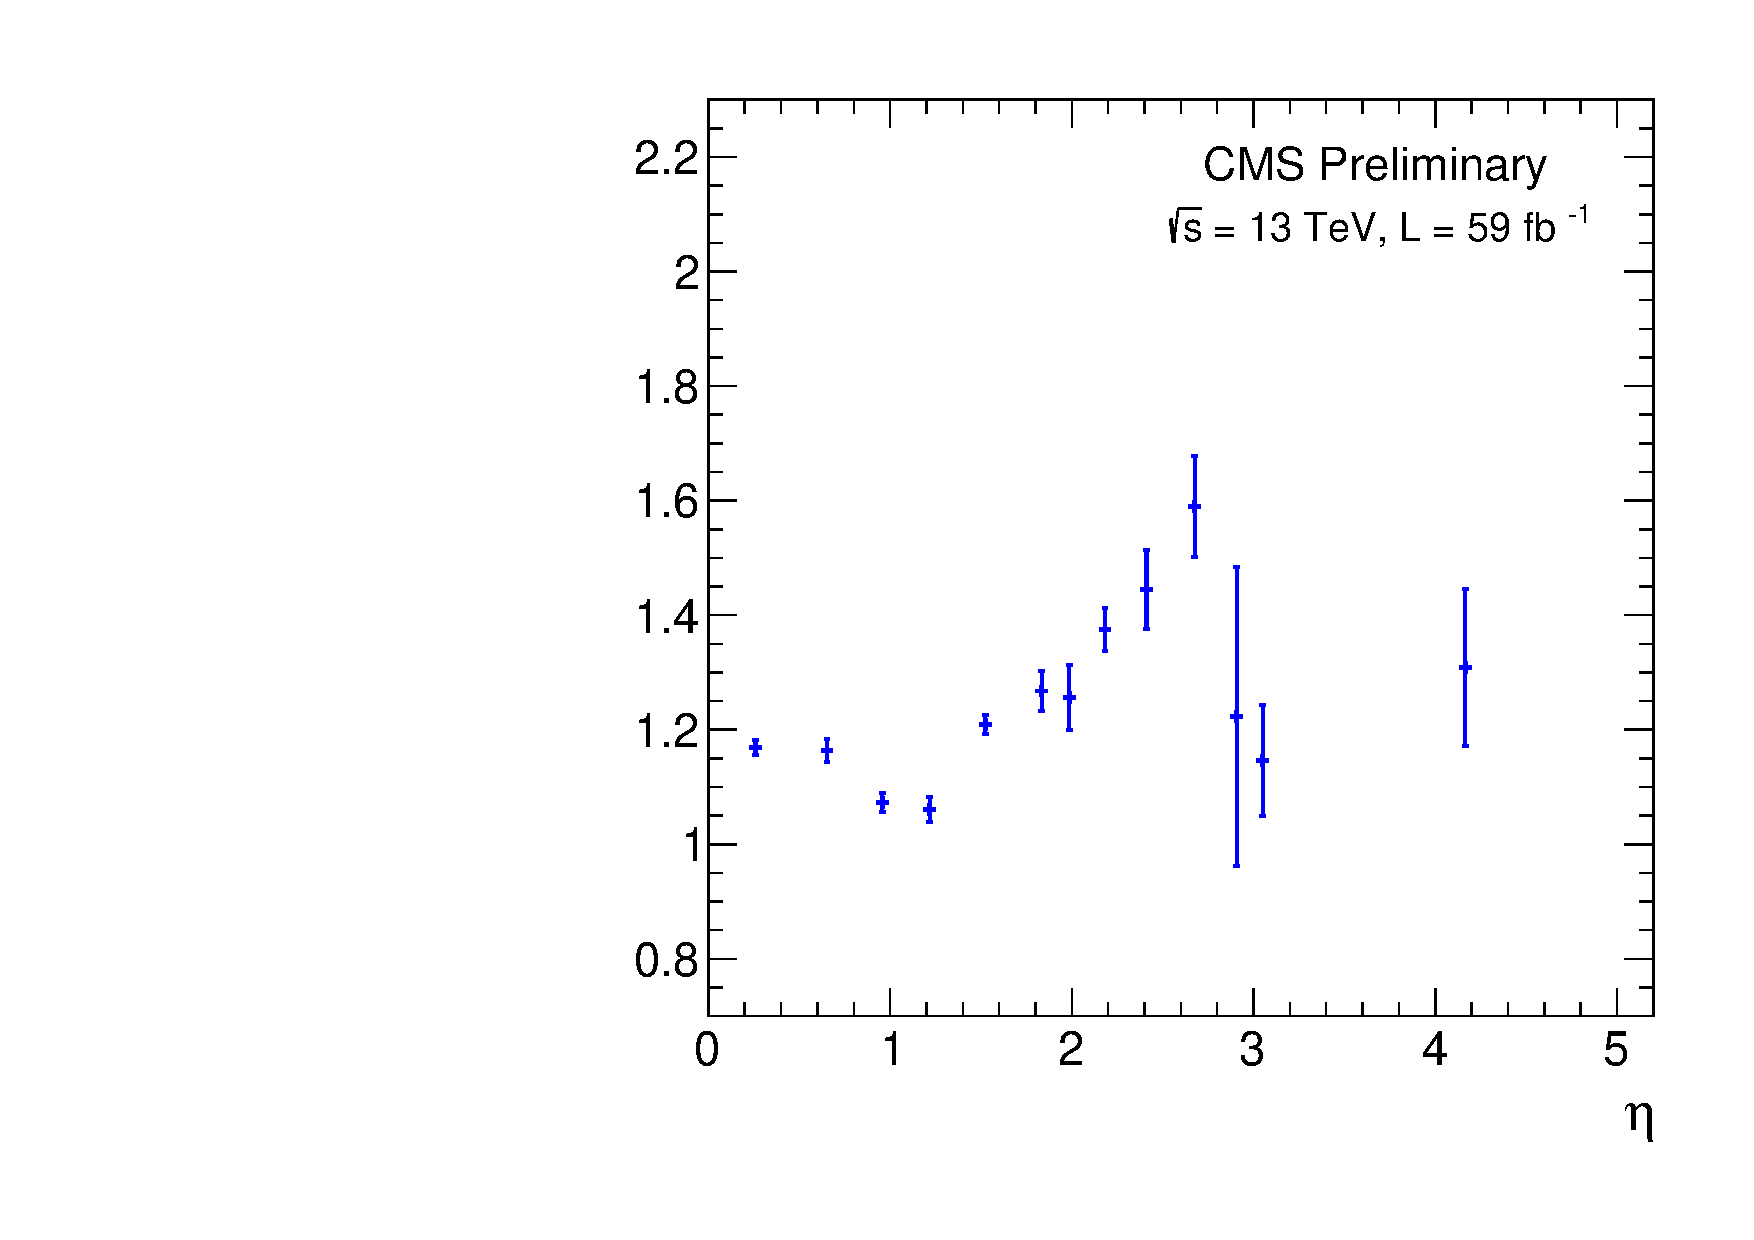
\includegraphics[width=.45\textwidth]{\PhDthesisdir/plots_and_images/my_plots/JERC/JER/Run2018ABCD/alpha_0_3/fine_eta_binning_Scale_factor_res_vs_ETA.tex}}
\hfill
\subcaptionbox{Facteurs correctifs utilisés par la collaboration lors du Run~II~\cite{CMS-DP-2020-019}.\label{fig-chapter-JERC-section-JER-subsec-results-CMS-DP-2020-019-JER_SF_RunII}}[.45\textwidth]
{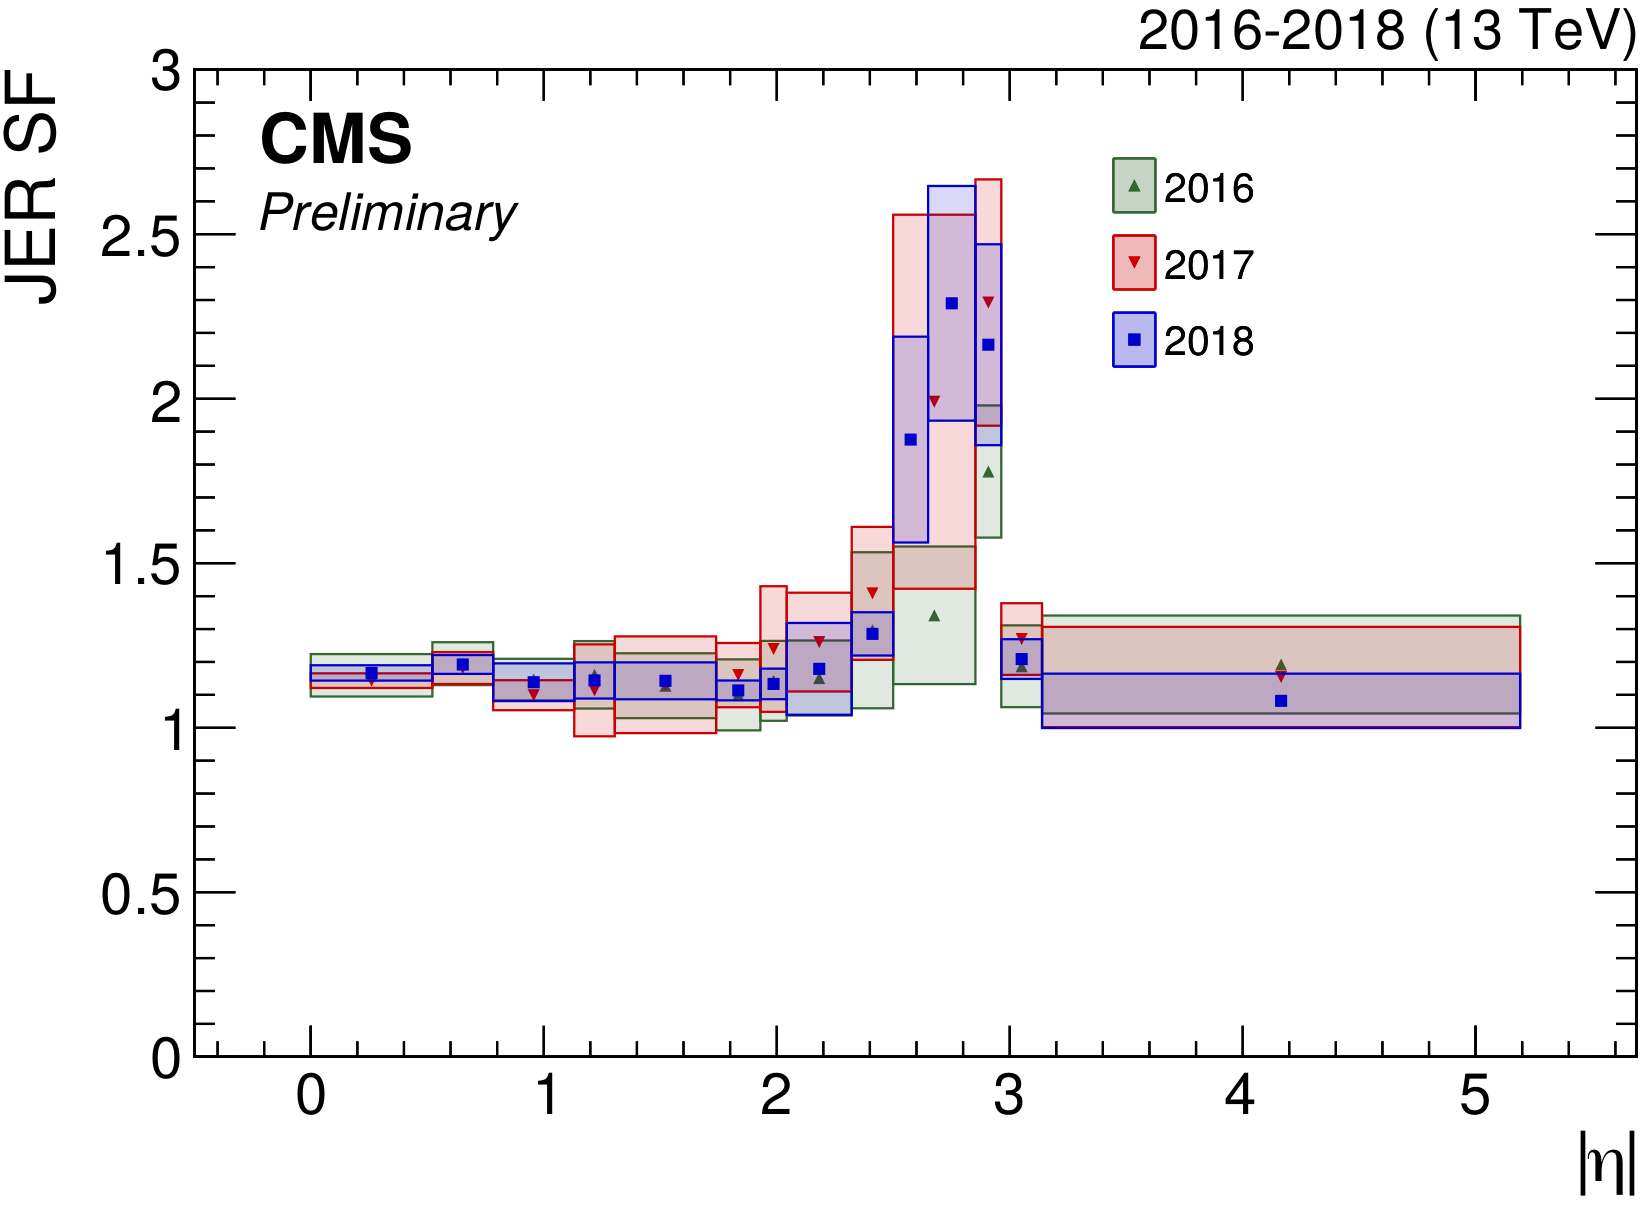
\includegraphics[width=.45\textwidth]{\PhDthesisdir/plots_and_images/from_CMS-DP-2020-019/JER_SF_RunII.png}}

\caption{Facteurs correctifs de la résolution en énergie des jets.}
\end{figure}